%%%%%%%%%%%%%%%%%%%%%%%%%%%%%%%%%%%%%%%%%
% University Assignment Title Page
% LaTeX Template
% Version 1.0 (27/12/12)
%
% This template has been downloaded from:
% http://www.LaTeXTemplates.com
%
% Original author:
% WikiBooks (http://en.wikibooks.org/wiki/LaTeX/Title_Creation)
%
% License:
% CC BY-NC-SA 3.0 (http://creativecommons.org/licenses/by-nc-sa/3.0/)
%
% Instructions for using this template:
% This title page is capable of being compiled as is. This is not useful for
% including it in another document. To do this, you have two options:
%
% 1) Copy/paste everything between \begin{document} and \end{document}
% starting at \begin{titlepage} and paste this into another LaTeX file where you
% want your title page.
% OR
% 2) Remove everything outside the \begin{titlepage} and \end{titlepage} and
% move this file to the same directory as the LaTeX file you wish to add it to.
% Then add \input{./title_page_1.tex} to your LaTeX file where you want your
% title page.
%
%%%%%%%%%%%%%%%%%%%%%%%%%%%%%%%%%%%%%%%%%
%\title{Title page with logo}
%----------------------------------------------------------------------------------------
%	PACKAGES AND OTHER DOCUMENT CONFIGURATIONS
%----------------------------------------------------------------------------------------

\documentclass[12pt]{article}
\usepackage[french]{babel}
\usepackage[T1]{fontenc}
\usepackage[utf8x]{inputenc}
\usepackage{amsmath}
\usepackage{graphicx}
\usepackage[colorinlistoftodos]{todonotes}
\usepackage{listings}
\usepackage{float}
\usepackage[justification=centering]{caption}
\usepackage[toc,page]{appendix}
\usepackage{url}
\usepackage{pgfplots}
\usepackage{hyperref} 
\usepackage{titlesec}
\usepackage[textwidth=6in]{geometry}
\usepackage[most]{tcolorbox}
\usepackage{lipsum}
\pagenumbering{roman}


\definecolor{eclipseStrings}{RGB}{42,0.0,255}
\definecolor{eclipseKeywords}{RGB}{127,0,85}
\colorlet{numb}{magenta!60!black}

\lstdefinelanguage{json}{
    basicstyle=\normalfont\ttfamily,
    belowcaptionskip=1\baselineskip,
    breaklines=true,
    frame=L,
    xleftmargin=\parindent,
    commentstyle=\color{eclipseStrings}, % style of comment
    stringstyle=\color{eclipseKeywords}, % style of strings
    numbers=left,
    numberstyle=\scriptsize,
    stepnumber=1,
    numbersep=8pt,
    showstringspaces=false,
    breakatwhitespace = true,
    escapechar        = *,
    string=[s]{"}{"},
    comment=[l]{:\ "},
    morecomment=[l]{:"},
    postbreak=\mbox{\textcolor{red}{$\hookrightarrow$}\space},
    literate=
        *{0}{{{\color{numb}0}}}{1}
         {1}{{{\color{numb}1}}}{1}
         {2}{{{\color{numb}2}}}{1}
         {3}{{{\color{numb}3}}}{1}
         {4}{{{\color{numb}4}}}{1}
         {5}{{{\color{numb}5}}}{1}
         {6}{{{\color{numb}6}}}{1}
         {7}{{{\color{numb}7}}}{1}
         {8}{{{\color{numb}8}}}{1}
         {9}{{{\color{numb}9}}}{1}
}


\setlength{\parskip}{0.2cm}%
\setlength{\marginparwidth }{2cm}

\begin{document}
\lstdefinestyle{customc}{
  belowcaptionskip=1\baselineskip,
  breaklines=true,
  frame=L,
  xleftmargin=\parindent,
  language=C,
  showstringspaces=false,
  basicstyle=\footnotesize\ttfamily,
  keywordstyle=\bfseries\color{green!40!black},
  commentstyle=\itshape\color{purple!40!black},
  identifierstyle=\color{blue},
  stringstyle=\color{orange},
}

\lstdefinestyle{customasm}{
  belowcaptionskip=1\baselineskip,
  frame=L,
  xleftmargin=\parindent,
  language=[x86masm]Assembler,
  basicstyle=\footnotesize\ttfamily,
  commentstyle=\itshape\color{purple!40!black},
}

\lstset{escapechar=@,style=customc}
% subsection


\titleclass{\subsubsubsection}{straight}[\subsection]

\newcounter{subsubsubsection}[subsubsection]
\renewcommand\thesubsubsubsection{\thesubsubsection.\arabic{subsubsubsection}}
\renewcommand\theparagraph{\thesubsubsubsection.\arabic{paragraph}} % optional; useful if paragraphs are to be numbered

\titleformat{\subsubsubsection}
  {\normalfont\normalsize\bfseries}{\thesubsubsubsection}{1em}{}
\titlespacing*{\subsubsubsection}
{0pt}{3.25ex plus 1ex minus .2ex}{1.5ex plus .2ex}

\makeatletter
\renewcommand\paragraph{\@startsection{paragraph}{5}{\z@}%
  {3.25ex \@plus1ex \@minus.2ex}%
  {-1em}%
  {\normalfont\normalsize\bfseries}}
\renewcommand\subparagraph{\@startsection{subparagraph}{6}{\parindent}%
  {3.25ex \@plus1ex \@minus .2ex}%
  {-1em}%
  {\normalfont\normalsize\bfseries}}
\def\toclevel@subsubsubsection{4}
\def\toclevel@paragraph{5}
\def\toclevel@paragraph{6}
\def\l@subsubsubsection{\@dottedtocline{4}{7em}{4em}}
\def\l@paragraph{\@dottedtocline{5}{10em}{5em}}
\def\l@subparagraph{\@dottedtocline{6}{14em}{6em}}
\makeatother

\setcounter{secnumdepth}{4}
\setcounter{tocdepth}{4}


\begin{titlepage}

\newcommand{\HRule}{\rule{\linewidth}{0.5mm}} % Defines a new command for the horizontal lines, change thickness here
\center % Center everything on the page

%----------------------------------------------------------------------------------------
%	HEADING SECTIONS
%----------------------------------------------------------------------------------------

\textsc{\LARGE SORBONNE UNIVERSITE}\\[1.5cm] % Name of your university/college
\textsc{\Large Rapport de stage en vu de l'obtention du master mention informatique parcours SAR}\\[0.5cm] % Major heading such as course name
\textsc{\large }\\[0.5cm] % Minor heading such as course title

%----------------------------------------------------------------------------------------
%	TITLE SECTION
%----------------------------------------------------------------------------------------

\HRule \\[0.4cm]
{ \huge \bfseries Sécurisation de la migration des machines virtuelles}\\[0.4cm] % Title of your document
\HRule \\[1.5cm]

%----------------------------------------------------------------------------------------
%	AUTHOR SECTION
%----------------------------------------------------------------------------------------

\begin{minipage}{0.4\textwidth}
\begin{flushleft} \large
\emph{Auteur:}\\
Salim Toufik \textsc{Nedjam}
\end{flushleft}
\end{minipage}
~
\begin{minipage}{0.4\textwidth}
\begin{flushright} \large
\emph{Encadrant:} \\
Antoine \textsc{BLIN}
\end{flushright}
\end{minipage}\\[2cm]

% If you don't want a supervisor, uncomment the two lines below and remove the section above
%\Large \emph{Author:}\\
%John \textsc{Smith}\\[3cm] % Your name

%----------------------------------------------------------------------------------------
%	DATE SECTION
%----------------------------------------------------------------------------------------

{\large \today}\\[2cm] % Date, change the \today to a set date if you want to be precise

%----------------------------------------------------------------------------------------
%	LOGO SECTION
%----------------------------------------------------------------------------------------

\includegraphics[scale=0.35]{include/logo_sorbonne.png}  % Include a department/university logo - this will require the graphicx package
\hspace{1.5cm}
\includegraphics[scale=0.20]{include/logo_gandi.png}\\ % Include a department/university logo - this will require the graphicx package

%----------------------------------------------------------------------------------------

\vfill % Fill the rest of the page with whitespace

\end{titlepage}

%-------------------------------------------------------------------------------
% BODY
%-------------------------------------------------------------------------------

\tableofcontents

\listoffigures
\newpage

\section*{Remerciements}

Je tiens à remercier les personnes travaillant au sein de l'équipe R\&D de GANDI, pour leur sympathie et leur disponibilité.
Mes remerciements s’adressent tout particulièrement à mon responsable de stage, Antoine Blin, je lui témoigne ici toute ma gratitude pour m'avoir guidé durant ces mois.


Je remercie Pierre Sens, qui a patiemment répondu à mes questions concernant ce stage.


Je souhaite remercier mon frère et ma sœur qui ont été toujours là pour moi et qui me servent de modèles dans ma vie.


Je souhaite exprimer toute ma gratitude et reconnaissance à mes parents, mes mots ne seraient jamais à la hauteur de l’amour et l’affection que vous m’avez témoignée tout au long de ma vie.
Cette dédicace serait pour moi, la meilleure façon de vous honorer et de vous montrer à quel point vous avez été magnifique, sans vous, je ne serrai jamais arrivé où je suis aujourd'hui. 

\newpage

\pagenumbering{arabic}
\setcounter{page}{1}
\section*{Introduction}
Actuellement, en dernière année de Master Systèmes et Applications Répartis à Sorbonne Université Science, le dernier semestre de mon cursus scolaire est consacré à la réalisation d’un stage au sein d’une société.
Il s’est déroulé du 08 mars au 08 septembre 2021 chez l’entreprise GANDI au sein de l'équipe Recherche et Développement.



Au fil des années, Linux est devenu le premier choix pour le développement de solutions sur le cloud.
De nombreux fournisseurs de clouds publics prospères utilisent la virtualisation Linux pour alimenter leurs infrastructures sous-jacente.
La consolidation et répartition des charges deviennent des éléments importants pour améliorer les capacités ces infrastructures complexes.
La migration de machines virtuelles est une des technique pour répondre à cette problématique.
Ces déplacements des VMs doivent se faire sans interruption de service et dans des délais très réduits afin de respecter la qualité globale des services.
Ces migrations imposent dès lors des responsabilités quant à l'intégrité des données transférées.
En effet, certaines précautions doivent être prises en amont pour qu’aucune incompatibilité ne survienne entre les machines concernées par le transfert.
Ce stage s’inscrit dans cette dynamique et cherche à sécuriser les mécanismes de migration des machines virtuelles afin de préserver l'intégrité des données migrées.


Nous allons maintenant aborder l’environnement technique au sein duquel mon travail a été effectué.
Nous verrons notamment les avantages de la virtualisation et détaillerons les principes de la migration des machines virtuelles.
Ensuite, nous aborderons les techniques de migration des machines virtuelles et décrirons les principales structures de données utilisées.
Nous parlerons par la suite du travail proposée, les problèmes rencontrés et les solutions apportées.
Enfin, nous allons évaluer le travail avec différents benchmarks.
% Domaine du stage (VM)
\newpage
\section{Contexte général}
Nous allons maintenant définir les raisons et les objectifs du projet.
Ensuite, nous découvrirons les cas d'usage et les avantages que propose la migration de machines virtuelles.
Enfin, nous citerons quelques problèmes et attaques que l'on peut relever lors d'une migration de machine virtuelle. 

\subsection{Rappel des objectifs}
Le projet SECPB s’inscrit dans le domaine du Cloud computing où des machines virtuelles sont utilisées pour assurer le déploiement de services logiciel auprès des utilisateurs finaux.
Les fournisseurs d’infrastructures (GANDI, SQUAD, Green Communications) sont chargés par leur client de déployer et d’assurer le bon fonctionnement de leurs solutions tout en fournissant des garanties de sécurité, de confidentialité et d’intégrité des données hébergées.
Dans le but d’assurer une meilleure gestion des pics de charge et des latences utilisateur, il a été envisagé d’effectuer un rapprochement entre les hébergeurs de machines virtuelles de telle sorte à ce qu’une machine virtuelle d’un client puisse être migrée entre les différentes infrastructures des fournisseurs.
Le gain de flexibilité de cette solution nécessite cependant la mise en œuvre de politique de sécurisation des données, faisant respecter le contrat qui lie les clients finaux avec leurs fournisseurs.
Il s’agit d’être capable de contrôler l’intégrité des machines virtuelles échangées en générant une empreinte desdites machines qui pourra être échangée de manière sécurisée entre les fournisseurs à travers une blockchain.

\subsection{Avantages de la migration de machine virtuelle}
Étant donné qu'un nombre croissant d'utilisateurs choisissent les centres de données dans le cloud pour héberger leurs applications,
la gestion efficace des machines virtuelles dans ces centres devient un problème majeur.
Par exemple, certains serveurs peuvent être surchargés, tandis que d'autres sont sous-utilisés, si un serveur tombe en panne, toutes les machines virtuelles qui s'y trouvent seront touchées.
Tous ces problèmes (comment répartir uniformément les tâches entre les serveurs, comment protéger les machines virtuelles contre les défaillances matérielles, etc.) sont résolus avec l'arrivée d'une technologie essentielle : la migration des machines virtuelles.
Une VM peut être déplacée d'un serveur à un autre, voire d'un centre de données à un autre.
La majorité des opérations de gestion du cloud sont prises en charge par la migration des machines virtuelles, telles que :

\begin{description}
    \item[La consolidation des serveurs]
    Les VM sont constamment créées et détruites dans un centre de données.
    En outre, certaines d'entre elles peuvent être suspendues ou inactives.
    Les VM seront donc mal réparties si les serveurs d'un centre de données ne sont pas correctement consolidés.
    Dans le cadre de la consolidation des serveurs, les machines virtuelles sont migrées pour des raisons énergétiques (en utilisant le moins de serveurs possibles) ou de communication (en plaçant les machines virtuelles qui communiquent beaucoup entre elles sur le même serveur pour réduire le trafic réseau).
    
    \item[Équilibrage de la charge]
    L'état de surcharge réduit non seulement la durée de vie d'un serveur, mais dégrade également la qualité de service (QoS).
    Par ailleurs, les serveurs fonctionnant en état de sous-charge entraînent un gaspillage d'énergie.
    La migration de machines virtuelles garantit que tous les serveurs d'un centre de données fonctionnent de manière égale, sans diminution de la qualité de service.
    Les charges peuvent même être équilibrées entre plusieurs centres de données géodistribués lorsque la migration de machines virtuelles est activée.

    \item[Maintenance matérielle sans temps d'arrêt]
    Les serveurs d'un centre de données peuvent avoir une forte probabilité de tomber en panne après une longue période de fonctionnement ou après être déjà tombés en panne.
    Ces serveurs peuvent être remplacés par de nouveaux serveurs en retirant toutes les machines virtuelles qui s'y trouvent et en les relançant après le remplacement de la machine. 
    Ceci s'applique également à la mise à niveau du matériel.

\end{description} 



\subsection{Problème lors des migrations de machine virtuelles}

La migration présente aussi de nombreuses failles de sécurité.
Les menaces de sécurité peuvent concerner les données, la gestion de contrôle et la migration.
Les personnes tierces peuvent provoquer des attaques passives et/ou actives, ce qui entraîne une dégradation des performances de la migration.
L'hyperviseur, sur lequel la migration est effectuée, est également vulnérable aux menaces de sécurité.
Cela pose de graves problèmes de confidentialité, d'authentification et de respect de la vie privée pour les données qui sont migrées entre deux serveurs.

Nous pouvons donner quelques exemples :

\begin{itemize}
    \item Les attaquants peuvent faire du snooping sur les données au cours de la migration de la machine virtuelle.  

    \item Les attaquants peuvent provoquer un dépassement de capacité du buffer en injectant du trafic indésirable dans le canal de communication, ce qui corrompt la mémoire du processus en cours d'exécution.
    
    \item Les attaquants peuvent exploiter la signature des entiers afin d'obtenir le contrôle de l'exécution du code en mode privilégié.
    
    \item Les attaquants peuvent modifier l'ordre des pages de mémoire transférées de la machine virtuelle source à la machine virtuelle de destination.   
\end{itemize}

Dans la suite de ce rapport nous allons nous concentrer sur les attaques qui affectent l'intégrité des données lors de la migration.

\newpage
\section{Contexte technique}
Nous allons maintenant aborder les différentes notions au cœur du sujet du stage en commençant par définir les concepts de base de la virtualisation. 
Ensuite, nous allons définir la migration dans le contexte des machines virtuelles ainsi que quelques types de migration qui sont définis dans la littérature.
Enfin, nous traiterons le processus de migration de machine virtuelle qui est mis en place dans QEMU.

\subsection{Virtualisation}
Nous allons maintenant aborder les principaux concepts de la virtualisation.
Dans un premier temps, nous allons définir la virtualisation, les hyperviseurs et nous évoquerons les différentes solutions existantes ainsi que leurs caractéristiques.
Ensuite, nous découvrirons la combinaison QEMU et KVM.
Enfin, nous détaillerons la pile de virtualisations dans le cas d'une virtualisation à l'aide de QEMU et KVM.

\begin{description}
    \item[La virtualisation] est une technologie qui consiste à faire cohabiter plusieurs systèmes d'exploitation.
    Elle permet ainsi d'exécuter un ou plusieurs systèmes d'exploitation sur une même machine qui se comportent comme des ordinateurs complets.
    La virtualisation nous garantit aussi l'isolation des OS et ainsi en cas de panne (logiciel) d'un des deux systèmes, l’autre n’en sera pas impacté.

    Il existe deux principales techniques de virtualisation qui peuvent être mises en place par le biais de respectivement un hyperviseur de type I et II :

    \item[Un hyperviseur] parfois appelé moniteur de machine virtuelle (VMM), a pour but de gérer l’accès aux ressources physiques par les systèmes d’exploitation invités.
    L'hyperviseur traite les ressources (CPU, mémoire et stockage) comme un pool qui peut être facilement réaffecté entre les machines virtuelles.

    \item[Un hyperviseur de type I] interagit directement avec le matériel du système ; il n'a pas besoin d'un système d'exploitation hôte.
    Il est mis en place directement sur un système bare metal.
    Les hyperviseurs de type 1 sont également appelés hyperviseurs Bare Metal, Embedded ou Native.\cite{kvmbook}
    C'est une solution de virtualisation complète, car elle permet d'utiliser les extensions de virtualisation matérielle Intel VT ou AMD-V par exemple.


    \item[Un hyperviseur de type II] est exécuté en userland (sur système d'exploitation hôte).
    Le principal avantage des hyperviseurs de type 2 est la large gamme de supports matériels, car le système d'exploitation hôte sous-jacent contrôle l'accès au matériel.
    Les hyperviseurs de type 2 sont également appelés hyperviseurs hébergés. \cite{kvmbook}
    \end{description}



\subsubsection{Choix d'un hyperviseur : QEMU}
QEMU est un émulateur de machine, il permet d'effectuer la virtualisation du matériel.
Tous les périphériques que le système d'exploitation invité voit, comme un clavier, une souris, une carte réseau, etc. sont des instances de code dans QEMU.
Beaucoup de ces périphériques sont basés sur les spécifications publiées pour le matériel physique disponible.
Les systèmes d'exploitation invités peuvent reconnaître ces périphériques grâce aux pilotes qui leur sont fournis.
QEMU peut fonctionner seul et émuler toutes les ressources de la machine virtuelle, son émulation logicielle le rend cependant extrêmement lent.

En plus d'imiter le matériel réel, QEMU crée également certains périphériques écrits spécifiquement pour les cas d'utilisation de la virtualisation.
Dans le cas de la combinaison QEMU/KVM, le framework virtio est utilisé pour créer ces périphériques.
Nous avons par exemple un périphérique réseau virtio-net, un périphérique bloc virtio-blk et ainsi de suite.
Les périphériques paravirtualisés ont l'avantage d'être conçus avec la virtualisation en tête, ils sont donc généralement plus rapides et plus faciles à gérer que l'émulation de périphériques réels.

Pour son fonctionnement, QEMU utilise plusieurs services du noyau Linux de l'hôte, comme l'utilisation des API KVM par exemple.

KVM est un hyperviseur de type 1 qui s'insère sous forme d'un module au noyau Linux pour le convertir en un hyperviseur.
KVM délègue la gestion de la mémoire, l'ordonnancement des processus, etc. au noyau Linux.
Cela signifie que toute amélioration du côté de Linux profite immédiatement à l'hyperviseur.

KVM expose son API à l'espace utilisateur via des ioctls, c'est par ce biais que QEMU utilise ses services.

Comme mentionné précédemment, l'émulation logiciel de QEMU le rend extrêmement lent. 
Pour surmonter ce problème, QEMU permet d'utiliser KVM afin de pouvoir utiliser les extensions de virtualisation du CPU physique.
QEMU s'exécute dans l'espace utilisateur et effectue une émulation matérielle virtuelle, tandis que KVM s'exécute dans l'espace noyau (hyperviseur de type 1), qui permet à un programme de l'espace utilisateur d'accéder aux fonctions de virtualisation matérielle des processeurs.


\subsubsection{Pile de virtualisation}
Les utilisateurs interagissent avec les machines virtuelles via l'une des nombreuses interfaces disponibles, comme virt-manager ou oVirt.
Ces logiciels interagissent à leur tour avec libvirt, qui fournit une API neutre vis-à-vis de l'hyperviseur pour gérer les machines virtuelles.

Pour les machines virtuelles QEMU/KVM, libvirt dialogue avec QEMU en utilisant les API fournies par QEMU.
Chaque machine virtuelle créée sur un hôte possède sa propre instance QEMU.
L'invité est exécuté dans le cadre du processus QEMU et chaque vCPU invité est vu comme un thread séparé dans les sorties top(1) et ps(1) de l'hôte.

Par la suite, QEMU s'interface avec Linux, en particulier le module KVM dans Linux, pour exécuter directement les machines virtuelles sur le matériel physique. 

\begin{figure}[H]
    \centering
    \includegraphics[scale=0.5]{include/pile.png}
    \caption{Représentation de la pile de virtualisation}
\end{figure}



\subsection{Techniques de migration}
En virtualisation, la migration de machines virtuelles consiste à déplacer l'état et les données d'une machine virtuelle, d'un hôte physique à un autre.
C'est une technique largement répandue au sein des centres de données des fournisseurs afin de gérer la répartition de charge et faire de la consolidation des serveurs.

La migration du contenu de la mémoire d'une VM d'un hôte physique à un autre peut être abordée de différentes manières.
Cependant, lorsqu'une VM exécute un service actif, il est important que ce transfert s'effectue d'une manière à minimiser le temps d'arrêt et le temps total de migration.

Le temps d'arrêt est la période pendant laquelle le service est indisponible parce qu'il n'y a pas d'instance de la VM en cours d'exécution ; cette période sera directement visible pour les clients de la VM en tant qu'interruption de service.

Le temps total de migration est la durée entre le moment où la migration est lancée et le moment où la VM originale peut potentiellement être mise hors service pour maintenance, mise à niveau ou réparation.

Il est plus facile de considérer les compromis entre ces exigences en généralisant le transfert de mémoire en trois phases :
\begin{description}
    \item[Phase de push]
        La VM source continue de fonctionner pendant que certaines pages sont envoyées à travers le réseau vers la nouvelle destination.
        Pour garantir la cohérence, les pages modifiées pendant ce processus doivent être envoyées à nouveau.
    \item[Phase de Stop-and-copy]
        La VM source est arrêtée, les pages sont copiées sur la VM de destination, puis la nouvelle VM est démarrée.
    \item[Phase de pull]
        La nouvelle VM s'exécute et, si elle accède à une page qui n'a pas encore été copiée, cette dernière est envoyée à travers le réseau depuis la VM source.
\end{description}

Bien que l'on puisse imaginer un schéma intégrant les trois phases, la plupart des solutions pratiques n'en retiennent qu'une ou deux. 
Deux techniques de migration de machines virtuelles existent:

\subsubsection{Migration à froid (non-live)}
La migration à froid est la stratégie la plus basique, il est cependant nécessaire de mettre la machine virtuelle hors tension afin de copier l'état de sa mémoire sur l'hôte cible.
Cette méthode a pour avantage de n'impliquer aucune erreur lors de la migration de la mémoire. En effet, la machine étant arrêtée tous les services ne sont plus disponibles et la mémoire ne sera pas modifiée par des processus.
Une fois migrée, la machine virtuelle reprendra son activité dans le même état que lorsqu'elle s'est arrêtée.
Elle comporte cependant un désavantage, à partir du moment où la machine est arrêtée, les services fonctionnant sous celle-ci ne seront plus disponibles durant toute la durée de la migration.
Cela pose évidemment des problèmes majeurs pour des applications nécessitant une haute disponibilité.
De plus, la mémoire étant transférée entièrement sur l'hôte cible, la migration à froid provoque un ralentissement du réseau. 

\subsubsection{Migration à chaud (live)}
La migration à chaud consiste à déplacer une machine virtuelle d'une machine hôte vers une autre machine sans la mettre à l'arrêt. 
Durant la migration, l'invité peut continuer d'utiliser la machine sans aucune différence.
Les connexions réseau restent actives et les applications continuent de fonctionner pendant le transfert de la machine virtuelle.
Cela signifie que de nombreuses variables entrent en jeu : bande passante du réseau, latence du réseau, disponibilité du stockage, etc.

Il y a une petite fenêtre pendant laquelle l'invité doit être arrêté pour que le nouvel hyperviseur prenne le relais et commence à exécuter l'invité.
Cela peut entraîner une dégradation des performances des applications de l'invité, et c'est la seule exposition de l'invité au processus de migration.

La migration à chaud est également appelée migration en direct.

Les deux types de migrations à chaud les plus connues sont :

\paragraph*{La migration pré-copie}
Elle combine une phase de push itérative suivie avec une phase d'arrêt et de copie généralement très courte.
Par \texttt{itératif}, nous entendons que la pré-copie se produit par cycles, dans lesquels les pages à transférer pendant le cycle sont celles qui ont été modifiées par des processus pendant le cycle précédent.

KVM expose à l'espace utilisateur une fonctionnalité gardant la trace des pages mémoires de l'invité qui ont été modifiées depuis la fois que celles-ci ont été demandées. 
Cette fonctionnalité permet notamment à QEMU d'envoyer uniquement les pages utilisées pendant le processus de migration.
La possibilité pour l'espace utilisateur, comme QEMU, de savoir quelles pages ont été modifiées depuis la dernière fois que ces données ont été demandées permet d'envoyer uniquement les pages sales.

Lors de la première phase de la migration, toutes les pages seront marquées comme sales.
La première itération transférera ainsi toutes les pages de mémoire.
Si les pages sales restantes calculées tombent sous la ligne de flottaison, la machine virtuelle peut être suspendue et les pages sales restantes ainsi que l'état des périphériques seront migrés en une seule fois.

Lorsque la mémoire de la machine virtuelle change fortement, le nombre des pages sales ne peuvent jamais descendre en dessous de la ligne de flottaison, ce qui implique que la migration ne peut donc jamais être achevée.
En d'autres termes, plus le nombre d'écritures en mémoire est important, plus la migration aura du mal à converger. 

\paragraph*{La migration on-demand (post-copie)}
En réponse aux problèmes ci-dessus, la méthode post-copie a été proposée.

Cette migration procède dans un premier lieu au transfert des structures de données essentielles vers la destination.
La VM de destination est ensuite démarrée, le reste des données est alors transféré depuis la machine source vers la machine virtuelle destinatrice à l'aide d'une combinaison de 4 techniques :
\begin{description}
    \item[Demand-paging] permet à l'hôte cible de demander une page mémoire manquante (Page fault) à l'hôte source, cette méthode implique inévitablement un ralentissement du système de par la lenteur du réseau.
    \item[Active-push] permet à l'hôte source d'envoyer à la cible les pages mémoire manquantes qui n'ont pas encore été demandées par l'hôte cible de manière pro-active.
    \item[Pre-paging] est un système permettant à l'hôte source de prédire la prochaine page fautive sur l'hôte cible en fonction des défauts de page récents.
    \item[Dynamic self balooning] permet quant à lui de réduire le nombre de transferts des pages non allouées.
\end{description}

La copie de pages sales du modèle pré-copie doit être terminée avant le démarrage de la machine virtuelle de destination, tandis que la copie de pages sales du modèle post-copie se poursuivra même après la reprise de la VM.

Cela permet de réduire considérablement le temps d'arrêt.
Dans la pratique, les performances après la migration sont susceptibles d'être dégradées jusqu'à ce qu'un ensemble considérable de pages ait été transférée.
Durant la migration, la machine virtuelle fera des erreurs sur une grande partie de ses accès à la mémoire, chacun d'entre eux initiant un transfert synchrone sur le réseau.

La migration en post-copie permet à la migration en direct de s'achever en un temps fini, indépendamment de la charge de la mémoire de la VM, ce qui constitue un outil fiable pour gérer la charge du serveur entre les hôtes.

Le principal inconvénient du mécanisme de post-copie est que toute interruption du réseau entraîne la perte de la VM.

\paragraph*{Migration hybride}
Le mécanisme de post-copie peut être utilisé pour aider la migration pré-copie.
En tant que telle, l'approche n'est ni purement pré-copie ni purement post-copie, mais un hybride qui combine les aspects des deux.
L'approche hybride est principalement utilisé lorsque la VM peut être migrée avec succès avec la technique de pré-copie, sans risque de perdre une instance en cas de défaillance réseau.

Le passage à la post-copie peut être effectué à tout moment s'il est conclu que la migration prend trop de temps et qu'elle ne convergera probablement pas dans un délai raisonnable.
Elle peut donc être utilisée comme solution de repli dans les scénarios où la VM est bloquée dans un état de migration en raison d'une forte activité mémoire.

Le principal inconvénient reste le même que pour la méthode post-copie, toute interruption du réseau entraîne la perte de la VM.

La combinaison de ces solutions de migration en direct offre le potentiel d'une gestion de la charge beaucoup plus fluide et flexible.


\begin{figure}[H]
    \centering
    \includegraphics[scale=0.5]{include/typemig.png}
    \caption{Représentation des différents types de migration}
\end{figure}

\subsection{Migration dans QEMU}
Nous allons maintenant aborder les différentes structures utilisées dans le cadre des migrations de machines virtuelles.
Ensuite, nous allons définir le protocole d'échange utilisé par les deux bouts de la migration.
Par la suite, nous décrirons le processus de migration de machine virtuelle avec les différents algorithmes qui sont mis en place.
Enfin, nous aborderons le sujet de la migration du disque.

\subsubsection{Structures de données dans QEMU}

Lors de la migration des objets, on peut distinguer deux types de périphériques :
\begin{description}
\item[Itératifs] concerne les périphériques avec un grand volume de données (RAM, disques ...).
\item[Non-itératifs (la plupart)] les données sont envoyées lorsque les CPUs sont stoppés
\end{description}

Chaque machine virtuelle a la capacité de sauvegarder un état complet et restaurable, y compris son vCPU, sa RAM et ses périphériques.

\subsubsection*{SaveState et SaveStateEntry}
Une structure de donnée de type \texttt{SaveStateEntry} est allouée pour chaque objet qui doit être migré.

Le principe de la migration des devices est de transférer chaque \texttt{SaveStateEntry} vers la machine de destination. 
Les informations contenues dans \texttt{SaveStateEntry} peuvent être des pages mémoire ou l'état des devices, on peut les distinguer par la variable \texttt{is\_ram}. 
Pour la machine virtuelle en cours d'exécution, ces informations peuvent changer à tout moment.

Les \texttt{SaveStateEntry} sont insérées dans une liste globale \texttt{savevm\_state} de type \texttt{SaveState}. 
\begin{figure}[H]
    \centering
    \includegraphics[width=\textwidth]{include/savestate.png}
    \caption{Schéma des structures SaveState et SaveStateEntry}
\end{figure}

Les opérations de migrations de chaque objet peuvent être encodées de deux manières différentes :
\begin{description}
\item[Par une structure de type \texttt{SaveVMHandlers}] contenue dans le champs `ops` du \texttt{SaveState} qui contient un ensemble de pointeurs de fonctions utilisé au cours du processus de migration.
\item[Par une structure de type \texttt{VMStateDescription}] contenue dans le champs `vmsd` qui permet d'encoder de manière générique n'importe quel périphérique en structure de données en C.
\end{description}

\subsubsection*{SaveVMHandlers (Legacy)}
\texttt{SaveVMHandlers} modélise les opérations à effectuer pour migrer un objet, ces fonctions s'occupent d'écrire et de récupérer dans une zone mémoire (opaque) l'intégralité de l'état du périphérique.
Chaque périphérique doit enregistrer au moins deux fonctions, une pour sauvegarder l'état et une autre pour le charger.
Voici un exemple d'initialisation de la structure pour la migration de la RAM.

\begin{lstlisting}[caption={Exemple d'une structure de donnée SaveVMHandlers},captionpos=b]
static SaveVMHandlers savevm_ram_handlers = {
    .save_live_setup = ram_save_setup,
    .save_live_iterate = ram_save_iterate,
    .save_live_complete_postcopy = ram_save_complete,
    .save_live_complete_precopy = ram_save_complete,
    .save_live_pending = ram_save_pending,
    .load_state = ram_load,
    .cleanup = ram_migration_cleanup,
};
\end{lstlisting}

\subsubsection*{VMStateDescription}
\texttt{VMStateDescription} décrit un VMState, il permet d'encoder de manière générique un ensemble de données à envoyer.
En d'autres termes", \texttt{VMState} est l'état du périphérique dans le modèle de périphérique QEMU.
Chaque état de périphérique a une structure.
La fonction principale d'un \texttt{VMStateDescription} est d'aider QEMU à juger pendant la migration, quels membres de la structure \texttt{VMState} doivent être migrés.
Pour qu'un device puisse être inclut dans une sauvegarde elle doit implémenter l'interface \texttt{VMStateDescription}, qui va contenir tous les champs nécessaires qui devrons être restaurés.
Prenons l'exemple de l'implémentation de IOMMU (Input-Output Memory Management Unit) :

\begin{lstlisting}[caption={Exemple d'une structure de donnée VMStateDescription},captionpos=b]
static const VMStateDescription vtd_vmstate = {
    .name = "iommu-intel",
    .version_id = 1,
    .minimum_version_id = 1,
    .priority = MIG_PRI_IOMMU,
    .post_load = vtd_post_load,
    .fields = (VMStateField[]) {
        VMSTATE_UINT64(root, IntelIOMMUState),
        VMSTATE_UINT64(intr_root, IntelIOMMUState),
        VMSTATE_UINT64(iq, IntelIOMMUState),
        VMSTATE_UINT32(intr_size, IntelIOMMUState),
        VMSTATE_UINT16(iq_head, IntelIOMMUState),
        [ . . . ]
        VMSTATE_END_OF_LIST()
    }
};
\end{lstlisting}

Dans cet exemple, \texttt{VMStateDescription} expose tous les registres internes de l'IOMMU afin qu'ils soient automatiquement sauvegardés et restaurés lors de la migration.
Cette méthode est générique et ne nécessite pas d'écriture de fonction qui permet de sauvegarder ou de restaurer les données.


\texttt{VMStateDescription} contient un tableau de champs, chaque élément étant une structure \texttt{VMStateField}.
Chaque champ contient plusieurs éléments, dont le nombre est déterminé par \texttt{num/num\_offset}, et sa taille est déterminée par \texttt{size/size\_offset}.
La position de départ des éléments est déterminée par offset, dans l'espace pointé par le pointeur opaque.

\texttt{VMStateDescription} n'existe pas seul, mais fait partie de \texttt{SaveStateEntry}.
Mais toutes les structures \texttt{SaveStateEntry} n'ont pas vmsd.
Par exemple, dans les \texttt{SaveStateEntry} de "ram" et "block" le vmsd n'est pas disponibles, il est remplacé par des routines \texttt{SaveVMHandlers}. 
\begin{figure}[H]
    \centering
    \includegraphics[width=\textwidth]{include/VMDescription.png}
    \caption{Schéma de la structure VMStateDescription}
\end{figure}



\subsubsection{Protocole d'échange}
Tout échange d’informations repose nécessairement sur un ensemble de conventions partagées entre l'émetteur et le destinataire d'un message.
Il faut que l'un et l'autre sachent notamment à quel moment commence la communication, avec quelle procédure (pour l'interprétation des données) et à quel moment elle se termine.


Il existe différents protocoles de transport qui peuvent être utilisés pour le transport du flux :
\begin{description}
    \item[tcp] utilise les sockets tcp.
    \item[unix] utilise les sockets unix.
    \item[exec] utilise les standards stdin/stdout à travers un processus.
    \item[fd] utilise un descripteur de fichier déjà ouvert.
    \item[rdma] utilise le protocole RMDA, ce qui permet de réduire le stress sur le CPU.
\end{description}

Habituellement, la migration de la machine virtuelle contrôlée par libvirt utilise la migration fd, qui est un moyen pratique de migration.
Le descripteur de fichier est ouvert par l'application de plus haut niveau (libvirt), et QEMU est seulement responsable de l'envoi de données au descripteur.


Sur QEMU, le protocole d'échange envoie les données sous forme d'objet au sein d'un flux.
Chaque objet peut être envoyé en de multiples parties encapsulées au sein de sections délimitées par des constantes numériques afin de multiplexer l'envoi de parties d'objets.

\subsubsection*{QEMU Section}

La migration de mémoire de QEMU prend la section comme unité, et toutes les informations migrées sont encapsulées dans des sections pour être écrites dans le flux de sortie. 

Le format d'une section est indiqué ci-dessous. 

\begin{figure}[H]
    \centering
    \begin{tabular}{|c | c|} 
        \hline
        Type & Specifique au type\\ 
        \hline
    \end{tabular}
    \caption{Représentation du format d'une section QEMU}

\end{figure}

Le premier octet est le champ de type.
Le contenu suivant varie selon les sections.

Voici les différentes sections qui interviennent lors de la migration d'une VM :

\begin{figure}[H]
    \centering
    \includegraphics[scale=0.4]{include/section.png}
    \caption{Liste des différentes sections utilisées lors de la migration}
\end{figure}

\begin{description}
    \item[Configuration section]
    Cette section de la migration est spéciale.
    Il s'agit de la section de configuration.
    Comme son nom l'indique, sa fonction est de configurer la migration.
    Il s'agit d'une section de l'état des périphériques, indiquant le type de machine de la machine virtuelle source.
    Lorsque la destination analyse la section, elle compare le type de machine.
    Si les champs ne sont pas les mêmes, la migration n'est pas autorisée, ce qui limite la migration des machines virtuelles ayant des types de machine différents à la source et à la destination.
    \item[RAM start section]
    Cette section est également spéciale.
    Il s'agit des métadonnées de toute la mémoire migrée, y compris la taille totale de la mémoire de tous les \texttt{SaveStateEntry}, ainsi que la longueur totale des \texttt{RAMBlock} pointé par chaque sous-ensemble de mémoire \texttt{SaveStateEntry}.

    \item[RAM part section]
    Cette section correspond aux données de la RAM.

    \item[VMState section]
    Cette section décrit tous les champs d'état du périphérique migrés.

    \item[VMDescription section]
    Cette section est constituée d'une description JSON du contenu à des fins d'analyse uniquement.

\end{description}

\subsubsection{Processus de migration}

\paragraph*{Côté source}
Le début de la migration de la mémoire se trouve dans \texttt{migration\_thread()} et est divisé en 4 étapes : 

\subparagraph*{Initiation de la migration}
Dans l'étape d'initiation de la migration, l'en-tête de migration de la mémoire est envoyée pour marquer le début de la migration.
Les informations de l'en-tête de migration sont alors envoyées ainsi que le magic number et la version.
Cette section est configurée comme une information facultative, en fonction du type de machine.
\begin{lstlisting}[caption={Code responsable de la phase d'initiation},captionpos=b]
qemu_savevm_state_header()
{       
    qemu_put_be32(f, QEMU_VM_FILE_MAGIC);
    qemu_put_be32(f, QEMU_VM_FILE_VERSION);
            
    if (migrate_get_current()->send_configuration) {
        qemu_put_byte(f, QEMU_VM_CONFIGURATION);
        vmstate_save_state(f, &vmstate_configuration, &savevm_state, 0);
    }       
} 
\end{lstlisting}

\subparagraph*{Préparation de la migration}
Il existe une liste pour les pages de mémoire qui doivent être transférées \texttt{ram\_list.blocks}. 
L'étape de préparation de la migration fait principalement deux choses :
\begin{enumerate}
    \item Marquer toute la mémoire (les rajouter dans \texttt{ram\_list.blocks}).
    \begin{lstlisting}[caption={Différentes fonctions d'initialisation de la bitmap},captionpos=b]
        ram_init_all
            ram_init_bitmaps
                ram_list_init_bitmaps()
                memory_global_dirty_log_start()
                migration_bitmap_sync_precopy(rs)
    \end{lstlisting}

    \item Envoyer les noms et tailles de toutes les pages migrés.
    \begin{lstlisting}[caption={Code responsable de l'envoie des nom et tailles des pages migrés},captionpos=b]
        RAMBLOCK_FOREACH_MIGRATABLE(block) {
            qemu_put_byte(f, strlen(block->idstr));
            qemu_put_buffer(f, (uint8_t *)block->idstr, strlen(block->idstr));
            qemu_put_be64(f, block->used_length);
        }
    \end{lstlisting}
\end{enumerate}

\subparagraph*{Copie de la migration}
La phase de copie de migration consiste simplement à copier les données de la mémoire vers la destination.
Le processus est le suivant :
la dirty bitmap est parcouru afin de trouver une page qui a été changé depuis la dernière itération pour la transférer vers la destination.
\begin{lstlisting}[caption={Code responsable de la phase de copie},captionpos=b]
ram_save_iterate()
{
  	pages = ram_find_and_save_block(rs, false)
    found = find_dirty_block(rs, &pss, &again)
    if (found) {
        pages = ram_save_host_page(rs, &pss, last_stage);
    }
}
\end{lstlisting}

\subparagraph*{Fin de la migration}
La toute première implémentation de la ligne de flottaison dans QEMU était plutôt simpliste : s'il restait 50 pages sales ou moins à migrer, nous passions à l'étape de fin.
Ou, lorsqu'un certain nombre d'itérations s'étaient écoulées sans que l'on ait progressé vers un nombre de pages sales inférieur à 50.

Cela a bien fonctionné au départ, cependant il a fallu ajouter plusieurs nouvelles contraintes.

Une mise à jour de QEMU à permis de changer quelques paramètres au code pour que les conditions de passage de l'étape de copie à celle de fin soient configurable par les administrateurs de l'hôte et de l'invité.

Les administrateurs invités peuvent spécifier le temps d'arrêt maximum acceptable.
Dans notre code de l'étape de copie, nous vérifions combien de pages sont modifiés (sales) à chaque itération par l'invité et combien de temps il faut pour transférer les pages à travers le réseau.
Cela nous permet de dresser une estimation de la bande passante du réseau.
En fonction de cette estimation et du nombre de pages sales de l'itération en cours, nous pouvons calculer le temps qu'il faudra pour transférer les pages restantes.
Si ce temps est dans la limite acceptable, nous passons à l'étape de fin.
Sinon, une nouvelle itération est faite. \cite{redhat}

À la fin de l'étape de migration, il y a trois phases principales : suspendre le processeur, copier la mémoire restante ainsi que les différents états des périphériques et copier l'état de la VM.

Le graphique ci-dessous montre les différentes sections envoyées dans chaque phase:
\begin{figure}[H]
    \centering
    \includegraphics[scale=0.4]{include/summerize.png}
    \caption{Relation entre les différentes sections et les phases de la migration}
\end{figure}

\paragraph*{Côté destination}

Le processus central de la migration de destination est \texttt{qemu\_loadvm\_state()}, le processus est le suivant : 

\subparagraph*{Préparation de la migration}
Dans la phase d'initiation de la migration, les champs du magic number, de version et de configuration sont analysés et la fonction configuration est appelée en même temps. 
\begin{lstlisting}[caption={Code responsable de la phase de préparation},captionpos=b]

    /* magic */
    m = qemu_get_be32(f);

    /* version */
    v = qemu_get_be32(f);


    /* configuration section */
    if (migrate_get_current()->send_configuration)
        ret = vmstate_load_state(f, &vmstate_configuration, &savevm_state, 0);

\end{lstlisting}

\subparagraph*{Copie de la migration}
La logique principale de la copie de migration est dans \texttt{qemu\_loadvm\_state\_main}.
Dans cette fonction, le type de section est analysé à partir du flux.
Comme le format de la section est le même, la section peut être analysée de la même manière.
Les différents types de sections ont seulement une logique de traitement différente, comme ci-dessous : 
\begin{lstlisting}[caption={Code responsable de la phase de copie},captionpos=b]
qemu_loadvm_state_main()
{       
retry:
    while (true) {
    	/* section */
        section_type = qemu_get_byte(f);
          
        switch (section_type) {
        case QEMU_VM_SECTION_START:
        case QEMU_VM_SECTION_FULL:
            ret = qemu_loadvm_section_start_full(f, mis);
			[ . . .]
            break;
        case QEMU_VM_SECTION_PART:
        case QEMU_VM_SECTION_END:
            ret = qemu_loadvm_section_part_end(f, mis);
            [ . . .]
            break;   
        case QEMU_VM_COMMAND:
            ret = loadvm_process_command(f);
    		[ . . .]
            break;
        case QEMU_VM_EOF:
            /* This is the end of migration */
            goto out;
        default:
        [ . . .]
            goto out;
        }
    }
    [ . . .]
}

\end{lstlisting}

\subsubsection{Migration disque}
Il existe plusieurs fonctionnalités implémentées dans QEMU pour manipuler les périphériques de stockage et les données, alors que l'invité est en cours d'exécution.
\begin{description}
    \item[migrate -b] est la fonctionnalité traditionnelle de migration de disque dans qemu-kvm.
    Elle copie le contenu d'un périphérique de bloc dans le cadre du flux de migration en direct.
    Il s'agit d'une approche de pré-copie utilisant une dirty bitmap.

    \item[block-stream] peut être utilisé pour la migration pré et post-copie.
    Elle crée un nouveau fichier image qui utilise l'ancienne image disque comme fichier de sauvegarde.
    Le contenu du fichier de sauvegarde est copié dans la nouvelle image, à condition qu'aucun nouveau bloc n'a été écrit.
    Elle nécessite l'utilisation de NFS ou d'un autre mécanisme pour accéder à la fois à la nouvelle image et au fichier de sauvegarde en même temps.
    Cette méthode n'utilise pas le flux de migration en direct.

    \item[drive-mirror] le principe est de pré-copier le contenu du disque sur l'hôte de destination.
    Elle n'utilise pas de fichiers de sauvegarde, l'image de destination peut donc être de n'importe quel format d'image.
    Là encore, elle nécessite NFS ou un autre mécanisme pour accéder à la fois à la nouvelle image et à l'ancienne.
    Cette méthode n'utilise pas le flux de migration en direct.

    Un avantage de l'approche drive-mirror par rapport à block-stream est que la machine virtuelle peut continuer à s'exécuter sur l'ancienne image en cas de panne de courant ou de crash pendant la migration.
\end{description}


\subsubsubsection{Processus de migration du disque}
Nous allons nous intéresser à la migration traditionnelle (migrate -b) car c'est la seule qui utilise le même flux que la migration de la mémoire.
Dans ce cas, le disque est considéré comme un simple device, il utilise la même logique que la migration de la mémoire.
Il existe une structure \texttt{SaveVMHandlers} pour définir les routines qui permettent de migrer le contenue des blocs du disque.

\begin{lstlisting}[caption={SaveVMHandlers responsable de la migration du disque},captionpos=b]
static SaveVMHandlers savevm_block_handlers = {
    .save_setup = block_save_setup,
    .save_live_iterate = block_save_iterate,
    .save_live_complete_precopy = block_save_complete,
    .save_live_pending = block_save_pending,
    .load_state = block_load,
    .save_cleanup = block_migration_cleanup,
    .is_active = block_is_active,
};
\end{lstlisting}

\paragraph*{Côté source}
Nous allons maintenant définir les différentes phases de la migration du disque coté source.

\paragraph*{Préparation de la migration}
Cette phase permet d'initialiser toutes les structures de données qui vont être utilisées lors de la migration du disque.
Par la suite le même mécanisme de dirty bitmap est mis en place.
Au départ, tous les blocs sont marqués comme sale.

\begin{lstlisting}[caption={Code responsable de la phase de préparation},captionpos=b]
static int block_save_setup(){
    [ . . .]
    ret = init_blk_migration(f);
    [ . . .]
    /* start track dirty blocks */
    ret = set_dirty_tracking();
    [ . . .]
}
\end{lstlisting}


\subparagraph*{Copie de la migration}
Dans cette phase, QEMU commence à transférer les blocs de disque qui sont marqués comme sales.
Dans un premier temps, on commence par une phase pour transférer tous les blocs disque existants.
Puis on enchaîne par une phase Dirty qui permet de transférer seulement les blocs qui ont subi des écritures.

\begin{lstlisting}[caption={Code responsable de la phase de copie},captionpos=b]
static int block_save_iterate()
{
    [ . . .]
    /* control the rate of transfer */
    while (block_mig_state.read_done * BLK_MIG_BLOCK_SIZE <
           qemu_file_get_rate_limit(f) &&
           block_mig_state.submitted < MAX_PARALLEL_IO &&
           (block_mig_state.submitted + block_mig_state.read_done) <
           MAX_IO_BUFFERS) {

        if (block_mig_state.bulk_completed == 0) {
            /* first finish the bulk phase */
            if (blk_mig_save_bulked_block(f) == 0) {
                /* finished saving bulk on all devices */
                block_mig_state.bulk_completed = 1;
            }
        } else {
            /* Always called with iothread lock taken for
             * simplicity, block_save_complete also calls it.
             */
            qemu_mutex_lock_iothread();
            ret = blk_mig_save_dirty_block(f, 1);
            qemu_mutex_unlock_iothread();
        }
    }
    [ . . .]
}
\end{lstlisting}

\subparagraph*{Fin de la migration}
Le passage de la phase deux à la phase trois est la même que pour la migration de la mémoire.
Si le temps pour transférer les blocs restants est dans la limite acceptable, nous passons à l'étape de fin.
Dans cette phase, la machine virtuelle est gelée, et le transfert des derniers blocs dirty se fait.

\begin{lstlisting}[caption={Code responsable de la phase de fin},captionpos=b]
static int block_save_complete()
{
    [ . . .]
    /* we know for sure that save bulk is completed and
       all async read completed */
    [ . . .]
    do {
        ret = blk_mig_save_dirty_block(f, 0);
        if (ret < 0) {
            return ret;
        }
    } while (ret == 0);

    /* report completion */
    [ . . .]
}
\end{lstlisting}



\paragraph*{Côté destination}
La récupération des donnés côtés destination consiste en une phase décrite dans la fonction \texttt{block\_load()}.
Dans un premier temps, on récupère le nom du device et le numéro du secteur.
\begin{lstlisting}[caption={Code responsable de la récupération du nom du device et du numéro de secteur},captionpos=b]
    addr = qemu_get_be64(f);
       
    flags = addr & (BDRV_SECTOR_SIZE - 1);
    addr >>= BDRV_SECTOR_BITS;

    if (flags & BLK_MIG_FLAG_DEVICE_BLOCK) {
        /* get device name */
        len = qemu_get_byte(f);
        qemu_get_buffer(f, (uint8_t *)device_name, len);
        device_name[len] = '\0';
        blk = blk_by_name(device_name);
        [ . . .]
    }
\end{lstlisting}

Par la suite, on récupère les données pour mettre à jour le disque coté destination.
\begin{lstlisting}[caption={Code responsable de la récupération des données},captionpos=b]
    buf = g_malloc(BLK_MIG_BLOCK_SIZE);
    qemu_get_buffer(f, buf, BLK_MIG_BLOCK_SIZE);
\end{lstlisting}

\newpage
\section{Contribution}
Dans cette section, nous présentons la contribution faite dans le cadre du stage.
Nous commençons par lister le cahier des charges du stage.
Ensuite, nous allons parler de la contribution et expliquer les différents choix d'implémentation.


\subsection{Cahier des charges}
Dans cette section, nous allons définir le cahier des charges du projet.

\subsubsection{JSON}
La carte d’identité de la machine virtuelle est exprimée sous la forme d’un JSON contenant les empreintes des deux éléments permettant de caractériser une machine virtuelle afin d’assurer la propriété d’intégrité.\cite{cdc}
Elle contient trois éléments principaux :
\begin{description}
    \item[uuid]  L’identifiant alphanumérique de la machine virtuelle, chaque machine
    virtuelle disposant d’un identifiant unique.
    \item[type] Le type de migration effectué :
    \begin{description}
        \item[cold] Migration à froid de la machine virtuelle. La machine virtuelle est
        éteinte/suspendue et son image disque est migrée entre les deux fournisseurs.
        \item[lan] Migration à chaud avec disque dur partagé. La machine virtuelle
        est migrée sans interruption de service. Le disque dur est partagé
        (NFS, iSCSI...) entre la machine virtuelle source et destination, seule
        la mémoire est donc activement migrée.
        \item[wan] Le disque dur n'est pas partagé entre la machine virtuelle source et destination, ça migration est donc nécessaire ainsi que la mémoire.
    \end{description} 
    \item[fingerprints] Section contenant les empreintes devant être utilisées pour caractériser la VM. Elle contient deux sous-sections:
    \begin{description}
        \item[memory] Cette sous-section contient l’empreinte permettant d’identifier
        les données mémoire.
        
        \item[disk] Cette sous-section contient l’empreinte permettant d’identifier les
        données disques.

        Une empreinte est identifiée par un dictionnaire contenant deux couples de clef valeur :
        \item[algorithm] L’algorithme utilisé pour calculer l’empreinte.
        \item[hash]  L’empreinte effective du périphérique.
        Les deux sections memory et disk ne sont pas obligatoirement présentes selon le type de migration effectué :

        \begin{figure}[H]
            \centering
            \begin{tabular}{|c | c | c | c |} 
                \hline
                Présence & cold & lan & wan \\ 
                \hline
                memory & NON & OUI & OUI \\ \hline
                disk & OUI & NON & OUI \\ \hline
            \end{tabular}
            \caption{Tableau de types de migration}
        \end{figure}

    \end{description}

    \item[hypervisor] Une description de l’hyperviseur source et de la configuration nécessaire pour accueillir la machine virtuelle migrée.
    Elle contient trois sous-sections :

    \begin{description}
        \item[name] Le nom de l’hyperviseur source.
        \item[version] La version de l’hyperviseur source.
        \item[configuration] Une description de la configuration nécessaire à la migration. 
        Cette description varie selon les hyperviseurs et n’est donc pas normalisée.
    \end{description} 

\end{description}

Voici un exemple de la sortie souhaité:
\begin{lstlisting}[language=json,caption={Exemple de carte d'identité de migration},captionpos=b]
{
    "uuid": "oUXbdAEtCStygyfdzytRYfdy",
    "migration_type": "wan",
    "fingerprints": {
        "memory": {
            "algorithm": "sha256",
            "hash":"2b5326bed38bf8b344f4faddaaa80e1f6428   b844b384251e431ca1353248123b"
        },
        "disk": {
            "algorithm": "sha256",
            "hash":"e45ba2e4318f64ad7fedbcf666c481a34eba   12f4599b31dc21eac3242cc7a12a"
        },
    },
    "hypervisor": {
        "name": "kvm",
        "version": "5.2.50",
        "configuration": {
            "memory": 1024,
            "vcpus": 2,
            "disk": {
                "driver": {
                    "name": "qemu",
                    "bus": "virtio",
                    "file": "/var/images/vm.qcow2",
                    "if": "virtio"
                }
            }
        }
    }
}
\end{lstlisting}

\subsection{Solution}
Dans cette section, nous allons parler des différentes contributions du projet et du choix de nos implémentations.

\subsubsection{Calcul de l'empreinte de la machine virtuelle}
En vue de sécuriser l'intégrité des données échangées, la réalisation d'une empreinte de machine virtuelle met en exergue des problématiques de performances.
En effet, afin de minimiser les latences de migration, il est nécessaire de calculer le plus rapidement possible l’empreinte d’une machine virtuelle.
Celle-ci peut potentiellement manipuler un volume de données conséquent dont les données changent constamment.
Or, les fonctions de hash traditionnelles devant être exécutées lors de l'arrêt de la machine source engendrent des temps de calcul et des latences additionnelles qui sont prohibitives.\cite{usecase}

Les solutions de calcul de hash en mode flux permettent aussi de répartir le temps de calcul de l'empreinte pendant que la machine virtuelle est en cours d’exécution (Total time) et ainsi éviter de faire la totalité du calcul lors de la phase de downtime (l'arrêt de la machine source).

Nous avons choisi l'algorithme SHA-1 pour notre implémentation. 
Celui-ci propose une fiabilité suffisante et la vitesse de hash est supérieur à MD5 et SHA-256.

\subsubsection{Différentes approches de la résolution du problème}
Lors du processus de résolution de la problématique, il a fallu se confronter à l'analyse de la pile d'appels des fonctions pour transformer les données (Page de RAM, bloc de disque, état des périphériques ...) en un flux binaire qui serra transmis lors de la migration.
Il a fallu chercher le meilleur endroit dans cette pile d'appels de fonction pour faire le calcul du hash.\cite{usecase}

Ce graphique propose une vue simpliste des différentes portions ou le calcul de l'empreinte peut se faire.
\begin{figure}[H]
\centering
\includegraphics[scale=0.5]{include/placement.png}
\caption{Représentation graphique des différentes approches}
\end{figure}


\begin{description}
    \item[Partie 1] dans ce niveau sont envoyées les données (sous forme d'octet ou de bloc de données) de l'état des différents périphériques.
    
    Les avantages de faire le calcul de hash dans ce niveau sont :
    \begin{enumerate}
    \item Connaissance du type de données envoyé (device, ram, disque).
    \item Les données des headers de section ne sont pas inclues dans le calcul de hash, impliquant moins de temps CPU.
    \end{enumerate}
    Les inconvénients de faire le calcul de hash dans ce niveau sont :
    \begin{enumerate}
    \item Non-générique.
    \item Il est nécessaire de rajouter du code dans toutes fonctions qui envoient des données lors de la migration (chaque device, ram, disque).
    \item De nouveaux périphériques peuvent être ajoutés, impliquant du code supplémentaire pour le calcul de l'empreinte.
    \end{enumerate}
    
    \item[Partie 2] dans ce niveau les données transmises sont mises dans des vecteurs de tampons (iovec).
    Cela permet de travailler avec des blocs de données non-contigus, c'est-à-dire que les différents blocs de données peuvent être alloués séparément, pour être à la fin écrit dans un seul flux de donnée.
    
    Les avantages de faire le calcul de hash dans ce niveau sont :
    \begin{enumerate}
    \item Générique.
    \item Facile, peu de code à rajouter.
    \end{enumerate}
    Les inconvénients de faire le calcul de hash dans ce niveau sont :
    \begin{enumerate}
    \item Connaissance limitée du type de données envoyé (device, ram, disque).
    \item Les données des headers de section sont incluses dans le calcul de l'empreinte.
    \end{enumerate}
    \item[Partie 3] dans ce niveau les données sont aiguillés vers le bon protocole de transport, et les routines associées sont appelées pour transférer le flux de donnée.
    
    Les inconvénients de faire le calcul de hash dans ce niveau sont :
    \begin{enumerate}
    \item Les routines de tous les protocoles doivent être modifier pour inclure le calcul de l'empreinte.
    \item Les données étant bufferisées, il est n'est pas possible de distinguer le type des données (Disque, RAM) qui transite sans faire du calcul CPU supplémentaire pour chercher les différents headers de section.
    \end{enumerate}
    
    \end{description}
    
    \subsubsubsection{Approche retenue}
    L'approche implémentée lors du stage est celle de niveau 2.
    
    \begin{figure}[H]
    \centering
    \includegraphics[scale=0.5]{include/implem.png}
    \caption{Représentation graphique de approche retenue}
    \end{figure}
    
    L’implémentation consiste à hasher toutes les données qui sont envoyées par les différents devices (RAM, Disque, CPU ...). Il sera donc nécessaire de reconnaître les différents devices pour générer des hash différents : un pour la RAM et les différents périphérique et un autre dédié au disque.    
    
    Les différentes informations sur l'empreinte générée sont stockées dans une structure de donnée, déjà existante, \texttt{QEMUFile} qui sert à identifier le flux de migration (que ce soit de type rdma, fd, tcp ...).
    
    Après notre implémentation, la structure de donnée ressemble à :

\begin{lstlisting}[caption={Structure de donnée QEMUFile},captionpos=b]
    typedef struct QEMUFile {
        const QEMUFileOps *ops;
        const QEMUFileHooks *hooks;
        void *opaque;
    
        int64_t bytes_xfer;
        int64_t xfer_limit;
    
        int64_t pos; /* start of buffer when writing, end of buffer
                        when reading */
        int buf_index;
        int buf_size; /* 0 when writing */
        uint8_t buf[IO_BUF_SIZE];
    
        DECLARE_BITMAP(may_free, MAX_IOV_SIZE);
        struct iovec iov[MAX_IOV_SIZE];
        unsigned int iovcnt;
    
        int last_error;
        Error *last_error_obj;
        /* has the file has been shutdown */
        bool shutdown;
    
        //Fingerprint patch
        int is_wan;
        SHA_CTX hash_context;
        SHA_CTX hash_disk_context;
        QJSON *json_fingerprint;
        char *fingerprint_path;
        QemuUUID uuid;
    
    } QEMUFile;
\end{lstlisting}

Les différents ajouts sont :
\begin{description}
    \item[is\_wan] Permet de savoir si la migration de la machine virtuelle doit aussi procéder à la migration du disque.
    \item[hash\_context] Permet de calculer le hash de la mémoire et des différents périphériques.
    \item[hash\_disk\_context] Comme précédemment, ce champ permet de calculer le hash disque si \texttt{is\_wan} est à 1.
    \item[json\_fingerprint] Contient le contenu du fichier json qui serra généré à la fin de la migration et qui va contenir les différentes informations de l'empreinte de la machine virtuelle.
    \item[fingerprint\_path] Contient le chemin vers le fichier json en question.
    \item[uuid] Identifiant unique de la machine virtuelle.
\end{description}

Lors du lancement de la migration, ces différents champs sont initialisés.

\begin{lstlisting}[caption={Phase d'initialisation de la structure de donnée},captionpos=b]
    SHA1_Init(&(f->hash_context));
    if(f->is_wan)
        SHA1_Init(&(f->hash_disk_context));
    f->json_fingerprint = qjson_new();
\end{lstlisting}

Par la suite, chaque octet qui est transféré sur le réseau doit inévitablement faire évoluer (mettre à jour) l'empreinte de la machine virtuelle.
Vu que notre choix d'implémentation est au niveau 2, cela va nous permettre d'écrire moins de code (code générique) et ainsi être plus flexible lors des mises à jour de QEMU.

\begin{lstlisting}[caption={Mise à jour de l'empreinte de la machine virtuelle},captionpos=b]
SHA1_Update(&(f->hash_context), buffer, size);
\end{lstlisting}

À la fin de la migration (phase d'arrêt), il va falloir générer l'empreinte finale de la machine virtuelle et créer les fichiers JSON pour être sur de l'intégrité de la migration.

\begin{lstlisting}[caption={Action lors de la fin de la migration},captionpos=b]  
void fingerprint_process(QEMUFile *f) {
    unsigned char c[SHA_DIGEST_LENGTH];
    unsigned char hash[SHA_DIGEST_LENGTH*2];
    char *uuid = qemu_uuid_unparse_strdup(&(f->uuid));
    json_prop_str(f->json_fingerprint, "uuid", uuid);
    
    if (f->is_wan)
        json_prop_str(f->json_fingerprint, "migration_type", "wan");
    else
        json_prop_str(f->json_fingerprint, "migration_type", "lan");


    json_start_object(f->json_fingerprint, "fingerprints");
    
    SHA1_Final(c, &(f->hash_context));
    for (int i=0; i < SHA_DIGEST_LENGTH; i++) {
        sprintf((char*)&(hash[i*2]), "%02x", c[i]);
    }
    json_start_object(f->json_fingerprint, "memory");
    json_prop_str(f->json_fingerprint, "algorithm", "sha256");
    json_prop_str(f->json_fingerprint, "hash", (const char *)hash);
    json_end_object(f->json_fingerprint);

    if (f->is_wan) {
        SHA1_Final(c, &(f->hash_disk_context));
        for (int i=0; i < SHA_DIGEST_LENGTH; i++) {
            sprintf((char*)&(hash[i*2]), "%02x", c[i]);
        }
        json_start_object(f->json_fingerprint, "disk");
        json_prop_str(f->json_fingerprint, "algorithm", "sha256");
        json_prop_str(f->json_fingerprint, "hash", (const char *)hash);
        json_end_object(f->json_fingerprint);
    }

    json_end_object(f->json_fingerprint);

    qjson_finish(f->json_fingerprint);
    
    if(f->fingerprint_path) {
        FILE * fp;
        fp = fopen (f->fingerprint_path, "w+");
        fprintf(fp, "%s\n", qjson_get_str(f->json_fingerprint));        
        fclose(fp);
    }
}
\end{lstlisting}

Il faut prendre en compte que ces trois phases sont à la fois appliquées sur la machine source ainsi que la machine destination.


\subsubsubsection{Démarche de résolution de la problématique}
L'une des étapes les plus importante du stage a été d'analyser le code de la migration de QEMU ainsi que des différentes structures des données et leurs interactions avec l'intégrité du système.
En effet, il a fallu suivre l'acheminement des données de leur envoi depuis différents devices jusqu'à leur réception par la machine virtuelle destination.
Afin de vérifier que les données envoyées (source) et reçues (destination) soient équivalentes.

Dans un premier temps, nous avons récupéré chaque donnée envoyée par les périphériques à travers des sondes.
Ces sondes ont pour but de récupérer et écrire chaque octet sur un fichier.
À la fin de la migration, nous aurons deux fichiers : l'un qui représente les données envoyées par la machine virtuelle source et l'autre les données reçues par la machine virtuelle destination.
Le but final est de comparer les deux fichiers. 
Si aucune altération n'est survenue durant la migration, le contenu des deux fichiers seront équivalents générant alors deux hash identiques, résolvant notre problématique.
En vérifiant les hashs avec des outils de comparaison de code binaire (Hexcompare), nous nous sommes aperçu que quelques centaines de méga-octets de données était différent et changeait d'une migration à une autre.
Cela impliquait que les deux empreintes des VMs n'étaient pas équivalentes or la migration s'était déroulé sans altération de l'intégrité des données.
\begin{figure}[H]
\centering
\includegraphics[scale=0.2]{include/haxcompare.png}
\caption{Représentation graphique d'un diff entre les données envoyées et reçues.}
\end{figure}


Dans un second temps, on a utilisé des outils d'analyse de paquets (wireshark), afin de récupérer les données associées aux paquets envoyés et ceux reçus (payloads).
Après la récupération des payloads nous avons procédé à une comparaison entre les paquets envoyés et reçus.




Nous avons remarqué que certains périphériques mappaient directement la mémoire de l'utilisateur sur le flux réseau de la migration.
Il existait une fenêtre de temps entre le moment où les données étaient écrites sur le fichier et le moment où les données étaient envoyées sur le flux réseau.
Étant donné que la zone mémoire en question n'est pas protégée par un mutex, l'utilisateur pouvait modifier cette zone mémoire en plein transfert.
Cela engendrait des différences entre les fichiers générés côté source et destination.


Après que le contenu des deux fichiers était équivalent, nous avons modifié l'algorithme pour générer un hash des données au lieu de les écrire dans un fichier.
\subsection{Evaluation}
Dans cette section, nous présentons une évaluation approfondie de notre implémentation sur une grande variété de charges de travail.
Nous commençons par lister les différentes métriques pour tester la performance de notre contribution, par la suite nous allons décrire notre configuration de test, puis nous explorons en détail la migration de plusieurs charges de travail en détail.
Notez qu'aucune des expériences de cette section n'utilise les options d'optimisation citée en annexe, car nous avons souhaité mesurer les performances de base de notre système.


\subsubsection{Métrique de performances}
Une bonne stratégie de migration ne cherche pas seulement à déplacer une VM d'un endroit à un autre aussi rapidement que possible, mais doit aussi minimiser ses effets secondaires.
On peut mesurer l'efficacité d'un algorithme de migration grâce à ces métriques :

\begin{description}
\item[Temps total de migration]
Il s'agit de la durée entre le moment où la migration est initiée et le moment où la VM migrée est reprise sur le serveur de destination et qu'il ne reste aucune donnée à transférer depuis le site source.
\item[Temps d'arrêt (Downtime)] Il s'agit de la durée pendant laquelle la VM migrée est hors service.
Cette mesure détermine le degré de transparence de la migration pour les utilisateurs de la VM migrée.
Pour une migration non live, le temps total de migration est égal au temps d'arrêt.
\item[Trafic réseau total]
Cette mesure représente le total des données transférées pendant la migration.
Il s'agit d'une mesure critique lorsque la machine virtuelle migrée exécute un service à forte intensité de réseau, car elle se disputera la bande passante du réseau avec le processus de migration.
\end{description}

Les seules métriques nous permettant d'analyser les performances de notre solution sont le temps total et le temps d'arrêt.
En effet, le trafic réseau total n'est pas prise en compte pour analyser les performances de notre implémentation, car notre modification ne transfère aucune donnée sur le flux de la migration.


\subsubsection{Machine de test}
Nous effectuons des migrations de test sur une machine en local pour mieux observer l'impact de notre algorithme de hash avec comme bottleneck notre processeur.
La machine est équipée d'un processeur Intel® Core™ i7-1065G7 (8MB Cache, jusqu'a 3.9 GHz), d'une ram de 16GO avec une fréquence de 4267Mhz.

\subsubsection{Impact des charges de travail sur la migration}


Afin d'étudier un seul facteur, nous avons fixé des valeurs pour tous les paramètres, à l'exception des paramètres étudiés, et nous avons mesuré à la fois le temps d'arrêt et le temps total de migration à différents niveaux du paramètre étudié.

\begin{description}
\item[VM size]

Nous avons étudié le temps de migration des VM inactives avec VMSIZE configuré à 512 Mo, 1 Go, 2 Go, 4 Go et 8 Go de RAM.
Les machines virtuelles étaient inactives, aucun processus générateur de charge n'a été utilisé.

\begin{figure}[H]
\begin{minipage}{0.48\textwidth}
\centering
\includegraphics[width=1\linewidth]{include/down_vmsize.png}
\end{minipage}\hfill
\begin{minipage}{0.48\textwidth}
\centering
\includegraphics[width=1\linewidth]{include/total_vmsize.png}
\end{minipage}
\caption{Différence de downtime et du temps total pour la version par défaut et la version modifiée}
\end{figure}

\item[Dirty rate]
Afin de s'appuyer sur les mécanismes de trappe et de table des pages du système d'exploitation, toutes les approches de migration de VM copient le contenu de la mémoire en pages.
Par conséquent, une page entière doit être migrée même si seulement une fraction de la page est écrite.
Nous avons testé cette hypothèse en modifiant quelques octets en utilisant un script générant des pages sales au sein de la machine virtuelle.
Ce programme prend en paramètre la vitesse de génération de nouvelles pages sales (Dirty rate).

Nous avons remarqué que si l'on dépasse un dirty rate de 30\% la migration dans les deux cas (avec et sans modification) n'arrive pas à converger.
Pour nos résultats nous avons pris des vitesses de 0\%, 10\% et 20\%.

\begin{figure}[H]
\begin{minipage}{0.48\textwidth}
\centering
\includegraphics[width=1\linewidth]{include/down_rate.png}
\end{minipage}\hfill
\begin{minipage}{0.48\textwidth}
\centering
\includegraphics[width=1\linewidth]{include/total_rate.png}
\end{minipage}
\caption{Différence de downtime et du temps total pour la version par défaut et la version modifiée}
\end{figure}


\end{description}

En comparant les figures, nous pouvons constater que le temps d'arrêt présente un comportement très différent de celui du temps de migration, bien que le premier fasse partie du second.
Cela n'est pas surprenant, car une utilisation accrue de la mémoire (plus de pages écrites à un rythme croissant) nécessite le transfert de plus de mémoire dans la phase d'arrêt et de copie.

Notre implémentation rajoute un overhead d'en moyenne de 10 ms, c'est une valeur plus qu'acceptable, car la limite décrite dans QEMU pour passer à la phase 3 est de 300 ms.

En terme de pourcentage, pour l'overhead en phase de downtime nous obtenons une valeur de 40\% en plus.
Ceci est principalement lié au calcul de hash finale qui doit être faite dans la phase de downtime.
Cela parait énorme, mais il faudrait un overhead de 10000\% pour atteindre les 300 ms limite.
Cependant, l'overhead en temps total est de l'ordre de moins de 1\%, cela veut dire que le temps de calcul de l'empreinte est presque inclus dans le temps de transfert du flux.
Il faut prendre aussi en compte que le transfert est fait en local avec donc le CPU comme bottleneck.
\subsubsection{Proposition d'optimisation}

\begin{description}
    \item[Calcul du hash dans un thread différent] Dans notre implémentation, la génération de l'empreinte de la machine virtuelle se fait sur le même fil d'exécution que l'envoi des données sur le réseau.
    Dans un système où le réseau est le bottleneck, l'overhead induit par le hachage des données et de leur envoi est négligeable par rapport au temps de transfert.    
    Nous pouvons gagner quelques millisecondes en ayant deux threads parallèles lors de la génération de l'empreinte de la machine virtuelle: l'un va calculer le hash des données et l'autre va transférer les données sur le réseau.
    \item[Hashage intelligent des pages dirty] Cette optimisation consiste à créer un cache avec un algorithme d'éviction LRU.
    Le but ici est de ne pas hasher les données qui sont constamment modifiées mais à la place d'inclure dans le calcul de l'empreinte seulement les pages/blocs qui n'ont pas été modifiées depuis un certain temps.
    L'optimisation se découpe en plusieurs points :
    \begin{itemize}
    \item En tête de liste nous aurons les pages qui ont été modifiées le plus récemment, qui ont donc une grande probabilité à être modifié à nouveau.
    \item En queue de liste nous aurons les pages qui sont les plus anciennement modifiées, et donc ont moins de chance d'être modifiées.
    \item Si une page est évincée de la liste alors son contenu sera hashé.
    \item À la dernière phase de la migration (la phase d'arrêt de la machine source) la liste pourra être parcouru et le contenu des pages dirty restantes sera hashé. 
    La machine source étant arrêtée, il est impossible que les données changent.
    \end{itemize}
    \item[Hashage intelligent des pages vides] Cette optimisation consiste à éviter de hasher les pages/blocs qui sont initialisés avec des zéros ainsi que les pages non utilisées.
    \item[Hashage des données plus fin] Cette optimisation consiste à éviter d'inclure le header des sections dans le calcul de l'empreinte de la machine virtuelle.
\end{description}
    Toutes ces optimisations ont pour but de réduire la quantité des données incluse dans la génération de l'empreinte de la machine virtuelle et ainsi réduire la pression sur le CPU. 
    Ces optimisations ont permis de réduire l'overhead de notre implémentation.
    
\newpage
\section*{Conclusion}
L’arrivée de la migration de machines virtuelles a rajouté une véritable plus value en ce qui concerne les services hébergés sur le cloud.
En effet, nous pouvons atteindre des durée d'uptime jamais vu auparavant, impactant directement la qualité de service.
Cependant, ces techniques ne sont pas sans failles pouvant altérer l'intégrité des données des machines virtuelles.

Nous avons pu, en utilisant la génération d'empreintes de machines virtuelles, garantir l'intégrité des données transférées à travers le réseau et ainsi éviter une l'altération de la machine pendant la migration.
Il a fallu prendre en compte le temps de génération d'empreintes pour ne pas dégrader le QOS ainsi que la bande passante réseau.

Ce stage a été très enrichissant à plusieurs points de vue.
J’ai pu, d’un point de vue interne, découvrir le fonctionnement d’un service de recherche et développement, et appris comment appréhender un problème complexe.
De plus, les nombreux problèmes auxquels j'ai été confronté m'ont demandé une certaine rigueur pour les résoudre.
J'ai également eu la possibilité d'étudier le fonctionnement interne de la migration des machines virtuelles, j'ai ainsi pu approfondir mes connaissances techniques dans le domaine de la virtualisation en général, mais aussi comment garantir l'intégrité d'une machine virtuelle migrée.
Nous pouvons imaginer différentes pistes pour optimiser l'overhead dû à la génération de l'empreinte de la machine virtuelle avec une gestion plus intelligente des pages de mémoire vide et dirty, ainsi que la prise en charge du multi-threading.
\newpage
\section*{Annexe}
\subsection*{Options de migration}
Qemu propose certaines optimisations pour aider la migration à ce dérouler d'une manière plus efficace en terme du volume des données transférer et ainsi avoir le temps d'absence de la machine virtuelle le plus faible possible sans impacter les performances de cette dernière.

\subsubsection*{Xor Based Zero Run Length Encoding}
La capability xbzrle a pour but de réduire le downtime ainsi que le temps total de la migration.
Elle est utile s'il existe sur la machine virtuelle des processus qui font des accès mémoire intensive.
Quand cette option n'est pas activée, la totalité de la mémoire serra transférée.
Cette technique a pour but de chercher les changements en mémoire qui ont été faits depuis la dernière itération de la transmission de la mémoire, les compresser, et les transmettre à la machine destination.
ce qui permet de réduire le volume des données transférées entre les deux bout de la communication.

Pour pouvoir trouver les zones en mémoire qui ont changé, la VM émettrice doit garder l'ancien état de la page dans un cache
avec un algorithme d'éviction LRU (la taille par default du cache est de 64 Mo), puis xbzrle encode le delta entre
les deux pages.
Du côté de la VM réceptrice, elle utilise le contenu de la dernière page reçu et xbzrle pour décoder le nouveau contenu de la page.

\includegraphics[width=\textwidth]{include/xbzrle}
Le delta est calculé avec un xor entre l'ancien et le nouveau contenu de la page, le résultat de ce xor est des suites de zéros et d'uns,
ces derniers sont compressés de la manière suivante:

\begin{itemize}
    \item une suite de zéros est représentée par sa taille.
    \item une suite d'uns est représentée par sa taille suivie des nouvelles données.
    \item la taille est encodée avec ULEB128.
\end{itemize}
\subsubsection*{Paramètres}
\begin{itemize}

 \item[$\bullet$]xbzrle-cache-size: Taille du cache utilisé par XBZRLE lors de la migration, il doit être multiple de la taille de la page cible et une puissance de 2.

\end{itemize}

source:  \url{docs/xbzrle.txt}

\subsubsection*{Compress}
La capability compress a pour but de réduire la taille des données transférées pendant la migration.
Cette option consiste à compresser chaque page de RAM avant de l'envoyer sur le réseau, du côté
réception la page serra décompressé pour restaurer les données d'origine.
Cela peut être utile si on a une bande passante limitée.
En compressant les pages, on peut s'attendre à réduire de 60\% des données transférer
ainsi que réduire le temps total de migration et le downtime respectivement de 70\% et 50\%.

Le point négatif de cette approche, c'est qu'on augmente drastiquement le temps CPU dus au thread de compression et de décompression.
et donc augmenter le temps de migration. Si l'on possède un algorithme de compression assez performant, on peut réduire le temps de migration en augmentant le nombre thread
Cette option consomme beaucoup de temps CPU dans un système ou le CPU est le bottleneck il faudrait plutôt l'éviter, par contre
sur un système ou la bande passante est faible et le CPU est adéquat il est plus préférable d'utiliser la compression sur plusieurs threads.
\newline
\newline

\begin{tikzpicture}[scale=1]
    \node[align=center] at (1,1) {Get dirty \\ page};
    \draw [thick,decorate,decoration={brace,amplitude=6pt,raise=0pt}] (0,0.15) -- (2,0.15);

    \node[align=center] at (4.5,1) {Zero page \\check};
    \draw [thick,decorate,decoration={brace,amplitude=6pt,raise=0pt}] (2.5,0.15) -- (6,0.15);

    \node[align=center] at (10,1) {Send data};
    \draw [thick,decorate,decoration={brace,amplitude=6pt,raise=0pt}] (6.5,0.15) -- (13,0.15);

    \draw [thick,-] (0,0) -- (13,0);

\end{tikzpicture}
\captionof{figure}{Sans (dé)compression.}


\begin{tikzpicture}[scale=1]
    \node[align=center] at (1,1) {Get dirty \\ page};
    \draw [thick,decorate,decoration={brace,amplitude=6pt,raise=0pt}] (0,0.15) -- (2,0.15);

    \node[align=center] at (4.5,1) {Zero page \\check};
    \draw [thick,decorate,decoration={brace,amplitude=6pt,raise=0pt}] (2.5,0.15) -- (6,0.15);

    \node[align=center] at (8,1) {Compress page};
    \draw [thick,decorate,decoration={brace,amplitude=6pt,raise=0pt}] (6.5,0.15) -- (10,0.15);

    \node[align=center] at (11.5,1) {Send data};
    \draw [thick,decorate,decoration={brace,amplitude=6pt,raise=0pt}] (10.5,0.15) -- (13,0.15);

    \draw [thick,-] (0,0) -- (13,0);

\end{tikzpicture}

\captionof{figure}{Avec (dé)compression.}


\begin{tikzpicture}[scale=1]

    \node[align=center] at (1,1) {Get dirty \\ page};
    \draw [thick,decorate,decoration={brace,amplitude=6pt,raise=0pt}] (0,0.15) -- (2,0.15);

    \node[align=center] at (4.5,1) {Zero page \\check};
    \draw [thick,decorate,decoration={brace,amplitude=6pt,raise=0pt}] (2.5,0.15) -- (6,0.15);

    \node[align=center] at (7.5,1) {Compress page\\with multithread};
    \draw [thick,decorate,decoration={brace,amplitude=6pt,raise=0pt}] (6.5,0.15) -- (9,0.15);

    \node[align=center] at (10.5,1) {Send data};
    \draw [thick,decorate,decoration={brace,amplitude=6pt,raise=0pt}] (9.5,0.15) -- (12,0.15);

    \draw [thick,-] (0,0) -- (12,0);

\end{tikzpicture}

\captionof{figure}{Avec multi-thread (dé)compression.}


\subsubsection*{Paramètres}
\begin{itemize}

    \item[$\bullet$] compress-level: Niveau de compression:
        \begin{itemize}
            \item niveau 0: Pas de compression.
            \item niveau 1: Meilleure vitesse de compression.
            \item niveau 9: Meilleur ratio de compression.
        \end{itemize}

    \item[$\bullet$] compress-threads: Nombre de thread de compression.
    \item[$\bullet$] decompress-threads: Nombre de thread de décompression.
    \item[$\bullet$] compress-wait-thread: Donne la démarche à suivre si tous les thread de compression sont utilisés, Si à true (par défault), il faudra attendre qu'un thread devienne libre; sinon, on envoie la page sans compression.
\end{itemize}

source:  \url{docs/multi-thread-compression.txt}

\subsubsection*{Auto converge}
Certains workload ont tendance à salir la mémoire plus rapidement que le taux de transfert.
Malgré quelques améliorations récentes (et l'utilisation de cartes réseau 10Gb entre les hôtes) la migration peut ne pas converger.
\\

Pour résoudre ce problème, l'option autoconverge permet de ralentir le CPU en interdisant
explicitement aux VCPU de passer beaucoup de temps dans la VM, cela permet de valider la condition de passage
à la phase 3 de la migration plus rapidement (phase d'arrêt).

\subsubsection*{Paramètres}
\begin{itemize}
    
 \item[$\bullet$]throttle-trigger-threshold: Le ratio entre bytes\_dirty\_period et bytes\_xfer\_period
                              pour activé la dégradation des performances.
                              Valeur par défault est de 50 (pourcentage).

 \item[$\bullet$]cpu-throttle-initial: Le pourcentage initial de la dégradation des performances si auto-converge est activé.


 \item[$\bullet$]cpu-throttle-increment: L'increment du pourcentage des performence à reduire si on voit que la migration ne converge pas.

 \item[$\bullet$]max-cpu-throttle: Pourcentage maximum de la dégradation, par défault à 99.
\end{itemize}

source:  \url{https://wiki.qemu.org/Features/AutoconvergeLiveMigration}

\subsubsection*{Postcopy ram}
La Postcopy est également une méthode de migration dynamique populaire.
Par rapport à la pré-copie, la migration post-copie est plus rapide et peut presque établir une connexion transparente entre la source et la destination de la migration.
Pour les machines virtuelles avec de grandes quantités d'opérations de lecture et d'écriture de mémoire, surtout si la bande passante de migration est limitée, la post-copie est une méthode plus efficace pour la migration à chaud.

En termes simples, la post-copie consiste d'abord à transférer l'état du processeur existant, les registres et, éventuellement, la mémoire non-paginable (mémoire qui ne sera ni échangée ni déplacée en mémoire) de la machine virtuelle vers le serveur de destination.
Par la suite, la machine virtuelle est démarrée sur le serveur de destination.
Dans le même temps, le serveur source enverra également dynamiquement la mémoire restante vers le serveur de destination.
Mais lorsque la machine virtuelle utilise la mémoire qui n'a pas été transférée, une page-fault sera déclenchée.

La méthode post-copy gère ces pages-fault en se basant sur le mécanisme du noyau linux 'userfaultfd'.
userfaultfd permet à la machine cible d'obtenir les informations de la dite page via le descripteur de fichier fd dans l'espace utilisateur (espace utilisateur).
En termes simples, lorsque la machine virtuelle appelle la mémoire qui n'a pas été transférée sur le serveur de destination, userfaultfd peut accéder au serveur source pour extraire ces informations de mémoire et les transférer vers le serveur de destination pour permettre à la machine virtuelle de continuer à fonctionner.

\includegraphics[width=\textwidth]{include/Postcopyflow}
\captionof{figure}{List d'appels suite à un page-fault}


La pression de lecture et d'écriture de la machine virtuelle sur la mémoire n'affectera pas le succès de la post-copie, mais une fois la migration de la machine virtuelle terminée, si la pression de lecture et d'écriture sur la mémoire est importante, userfaultfd sera appelé fréquemment, ce qui exercera une pression sur la bande passante du serveur et entraînera également une dégradation des performances de la machine virtuelle.
\\

source: 
\begin{itemize}
    \item \url{https://wiki.qemu.org/Features/PostCopyLiveMigration}
    \item \url{https://en.wikipedia.org/wiki/Live_migration#Post-copy_memory_migration}
\end{itemize}

\subsubsection*{Postcopy blocktime}
Blocktime est une métrique pour la migration en post-copy, elle montre combien de temps, le vCPU était en état de veille interruptible en raison d'une page-fault.
Cette métrique est calculée à la fois pour tous les processeurs virtuels en tant que valeur superposée et
séparément pour chaque processeur virtuel. Ces valeurs sont calculées du côté du serveur destination, elles sont utilisées pour calculer le downtime de la post-copy.

source: \url{docs/devel/migration.rst}

\subsubsection*{Multiple fds}
Cette option permet d'utiliser plusieurs fd pour procéder à la migration.
En utilisant un flux unique pour la migration, cela pose plusieurs problèmes:
\begin{itemize}
    \item Le processeur qui fait la réception est un goulot d'étranglement sur 10Gigabit et plus rapide
    \item Nous copions toutes les pages pour la migration, même lorsque nous pouvons envoyer directement
    \item Nous rendons les Transparent HugePages plus difficile à utiliser
\end{itemize}

L'idée ici est donc de diviser le flux de migration en deux, l'un pour le code actuel et l'autre pour le contenu des pages RAM. Cela évite complètement les copies.

Canal principal:
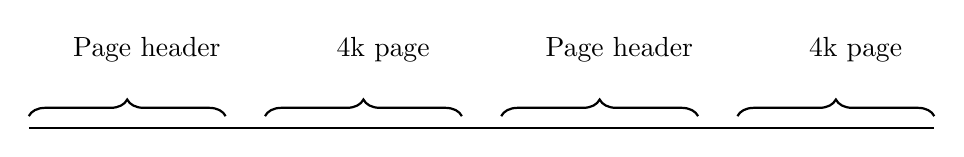
\begin{tikzpicture}[scale=1]
    \node[align=center] at (1.5,1) {Page header};
    \draw [thick,decorate,decoration={brace,amplitude=6pt,raise=0pt}] (0,0.15) -- (2.5,0.15);

    \node[align=center] at (4.5,1) {4k page};
    \draw [thick,decorate,decoration={brace,amplitude=6pt,raise=0pt}] (3,0.15) -- (5.5,0.15);

    \node[align=center] at (7.5,1) {Page header};
    \draw [thick,decorate,decoration={brace,amplitude=6pt,raise=0pt}] (6,0.15) -- (8.5,0.15);

    \node[align=center] at (10.5,1) {4k page};
    \draw [thick,decorate,decoration={brace,amplitude=6pt,raise=0pt}] (9,0.15) -- (11.5,0.15);

    \draw [thick,-] (0,0) -- (11.5,0);

\end{tikzpicture}

\captionof{figure}{Flux unique.}


Canal principal:
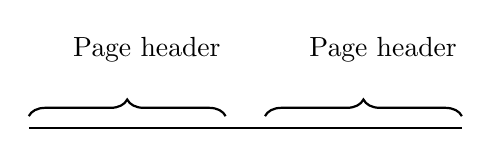
\begin{tikzpicture}[scale=1]
    \node[align=center] at (1.5,1) {Page header};
    \draw [thick,decorate,decoration={brace,amplitude=6pt,raise=0pt}] (0,0.15) -- (2.5,0.15);


    \node[align=center] at (4.5,1) {Page header};
    \draw [thick,decorate,decoration={brace,amplitude=6pt,raise=0pt}] (3,0.15) -- (5.5,0.15);


    \draw [thick,-] (0,0) -- (5.5,0);

\end{tikzpicture}


Canal secondaire:
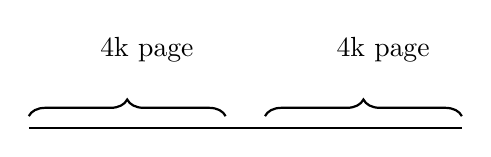
\begin{tikzpicture}[scale=1]

    \node[align=center] at (1.5,1) {4k page};
    \draw [thick,decorate,decoration={brace,amplitude=6pt,raise=0pt}] (0,0.15) -- (2.5,0.15);

    \node[align=center] at (4.5,1) {4k page};
    \draw [thick,decorate,decoration={brace,amplitude=6pt,raise=0pt}] (3,0.15) -- (5.5,0.15);



    \draw [thick,-] (0,0) -- (5.5,0);

\end{tikzpicture}

\captionof{figure}{Flux Multiple.}
\subsubsection*{Paramètres}
\begin{itemize}
 \item[$\bullet$]multifd-channels: Le nombre de flux utilisés pour la migration des données en parallèle. La par default est à 2.
\end{itemize}

source:  \url{https://wiki.qemu.org/Features/Migration-Multiple-fds}
\subsubsection*{RDMA pin all}
Le RDMA contribue à rendre votre migration plus déterministe sous forte charge, car la latence est nettement plus faible et le débit plus élevé que du TCP/IP classique, l'architecture d'E/S
RDMA réduit le nombre d'interruptions et copies de données en contournant la pile réseau hôte.

RDMA est actuellement disponible en deux versions : à la fois basée sur Ethernet (RoCE ou RDMA over Converged Ethernet) ainsi que sur Infiniband.

L'utilisation de RDMA pendant la migration nécessite de pin de la mémoire avec le matériel.
Cela signifie que la mémoire doit être physiquement présente avant que le matériel puisse transmettre cette mémoire à une autre machine.

Cette option permet d'épingler la totalité de la mémoire de la VM.



source:  \url{docs/rdma.txt}

\subsubsection*{X COLO}
Si cette option est activée, la migration ne se termine pas.
L'état du serveur émetteur serra migrer de manière constante vers le serveur destination, ce procédé est appelé COarse-Grain LOck Stepping.
c'est une technique de réplication de machine virtuelle, elle permet de fournir un «service non-stop» de tolérance aux pannes matérielles implémenté par logiciel indépendant de l'application.

La VM principale (PVM) et la VM secondaire (SVM) s'exécutent en parallèle.
Les paquets entrants du client ou du réseau externe sont reçus par le
nœud principal, puis transmis au nœud secondaire, de sorte que le PVM
et les SVM sont stimulés par les mêmes demandes.
Si les paquets de réponses de PVM et SVM sont identiques, ils sont envoyés immédiatement. Sinon, un point de contrôle VM (à la demande) est effectué.
source: \url{https://wiki.qemu.org/Features/COLO}


\subsubsection*{Autres options}
\begin{tabular}{ |p{3cm}|p{10cm}|  }
    \hline
    Nom de l'option& Description\\
    \hline
    \hline
    Zero blocks&Cette capability encode efficacement les blocs de zéros.\\
    \hline
    Release ram& Libérer les pages de RAM de la machine source migrée si l'option Postcopy ram est activée.\\
    \hline
    Block& Migrer également le contenu de tous les blocs device.\\
    \hline
    Pause before switchover& Suspendre la migration avant de sérialiser l'état des devices et avant de désactiver le block IO \\
    \hline
    Return path& La migration devra utiliser le chemin de retour même en post-copy\\
    \hline
    Dirty bitmaps& QEMU devra migrer les named dirty bitmaps\\
    \hline
    Late block activate& La destination devra ne pas activé les block devices à la fin de la migration\\
    \hline
    Ignore shared& QEMU ne va pas migrer la mémoire partagée \\
    \hline
    Validate uuid& Envoyer le UUID de la source pour permettre à la destination de vérifier la correspondance.\\
    \hline
   \end{tabular}
\\

source:  \url{https://github.com/qemu/qemu/blob/master/qapi/migration.json}

\include{parts/8-bibliography}



\clearpage

%\bibliographystyle{plain}
%\bibliography{bibliography}

\end{document}
